\documentclass{article}

%% [final] shows author names and removes the "Submitted to NeurIPS" footer.
%% NOTE: the EIML3 CFP states no anonymity policy. If OpenReview turns out to
%% require double-blind review, revert to \usepackage{neurips_2026} and strip
%% the author block.
\usepackage[final]{neurips_2026}

\usepackage[utf8]{inputenc}
\usepackage[T1]{fontenc}
\usepackage{hyperref}
\usepackage{url}
\usepackage{booktabs}
\usepackage{amsmath}
\usepackage{amssymb}
\usepackage{amsfonts}
\usepackage{amsthm}
\usepackage{graphicx}
\usepackage{float}
\usepackage{subcaption}
\usepackage{microtype}
\usepackage{nicefrac}
\usepackage{xcolor}
\usepackage{tikz}
\usetikzlibrary{arrows.meta}
%% decorations.pathreplacing + calligraphy are only needed for the OPTIONAL
%% gap brace in Figure 1's spec (section 7), which is not built. Add them back
%% if that brace is ever added.

% suppress the submission line numbers (no-op under [preprint]/[final])
\makeatletter
\@ifpackageloaded{lineno}{\nolinenumbers}{}
% [final] sets the footer notice to \@trackname, which is only defined by a
% track option (main / sglblindworkshop / ...). None is passed, so define it
% empty: authors still show, and there is no footer notice. To restore a
% workshop footer instead, pass [final,sglblindworkshop] and \workshoptitle{...}.
\providecommand{\@trackname}{}
\makeatother

\theoremstyle{plain}
\newtheorem{theorem}{Theorem}
\newtheorem{proposition}{Proposition}
\newtheorem{corollary}{Corollary}
\theoremstyle{definition}
\newtheorem{assumption}{Assumption}
\theoremstyle{remark}
\newtheorem{remark}{Remark}
\newtheorem{lemma}{Lemma}
\newcommand{\bpos}{b_{\mathrm{pos}}}
\newcommand{\btar}{b_{\mathrm{tar}}}         %% the target (silence-aware correct posterior)
\newcommand{\bstar}{\btar}                    %% legacy alias, was b*; now renders b_tar



\author{%
  Ali Khan \\
  Rutgers University \\
  \texttt{abk135@rutgers.edu} \\[2pt]
  Code: \url{https://github.com/akhan531/Control-On-LLMs}
}







%% =====================================================================
%%  Channels to Targets: A Closed-Form Coordinate System for
%%  Silence-Blindness in LLM Observers
%%
%%  EIML3 @ NeurIPS 2026  ·  4 pages excluding references
%%  Deadline 2026-08-29, 6:00 PM ET
%%
%%  SKELETON generated 2026-08-22 against eiml_paper_outline.md rev 3.
%%  Prose is drafted throughout. Section 2 is Ali's own. Everything else is a
%%  full draft to edit rather than a blank page. The abstract is deliberately
%%  empty and gets written last (item 87).
%% =====================================================================
%%
%%  AUTHORITIES, in precedence order:
%%    1. claims_to_evidence.md rev 4  -- every number and its population
%%    2. eiml_paper_outline.md rev 3  -- section numbering and structure
%%    3. PROVENANCE.md                -- what may be claimed about registration
%%    4. citation_ledger.md           -- bibliography
%%
%%  ITEM 66. Claim sentences and related-work characterizations are yours
%%  to type. Every strawman that falls under item 66 is tagged
%%      %% <ITEM66>
%%  Grep that tag before submitting. If any survive verbatim, item 66 has
%%  not been discharged.
%%
%%  WORDING RULES, binding:
%%    R1  Spans and universals, never singletons.
%%    R2  The universal is usually hiding behind the fraction. Lead with it.
%%    R3  State the population on every count.
%%    R4  "Frozen", "pre-registered", "pre-committed" NEVER unqualified.
%%        Ordering is not established for any artifact in this project.
%%        Kill conditions were fixed at a checkpoint before their test ran:
%%        that is a PROCESS claim and is labelled as one.
%%    R5  Significance goes at the CELL, never at the draw. Draw tallies are
%%        descriptive counts with ATTEMPTED denominators and carry no p-value.
%%
%%  BANNED NUMBERS (claims_to_evidence.md sec 7). Grep each one before
%%  submitting; none may appear anywhere in this file:
%%    962 · 176 · 206 · p ~ 0.004 · "5/5" occupancy · 2 of 210 ·
%%    pooled 27/79/197/22 · "~100%" gap closure · "8 of 11 non-control cells" ·
%%    "five configurations respond to record length" · "4 of 5" cross-regime ·
%%    "~7,050" as a bare total · "all failures are PARSE in the deepseek family" ·
%%    "all seven configurations agreed" on the W1 bands
%%
%%  TWO LIVE NUMBER COLLISIONS. Disambiguate at first use or drop one:
%%    - two different 16s in Example 1's lean-baseline neighbourhood
%%      (BEY escapes among excluded draws; gated failures in RULEDCTRL)
%%    - two unrelated 5/5s in Example 2
%%
%%  PAGE BUDGET (pages):
%%    title+abstract 0.25 | S1 0.50 | S2 0.75 | S3 0.65 | S4 0.60
%%    S5 0.60 | S6 0.40 | S7 0.25 | TOTAL 4.00
%%  Objects: 2 figures, 2 tables, 3 numbered equations, 1 proposition, 1 lemma.
%%
%%  CUT BRANCH at 3.5 pages, in this order:
%%    Table 2 -> appendix, S6 becomes prose; blind spots 5 and 6 merge
%%    (KEEP the one-bin sentence, CUT the span-pooling sentence);
%%    Figure 1 goes; S3 band-gap paragraph -> one sentence; S7 -> three
%%    sentences. NOTHING IN S2 MOVES.
%% =====================================================================


%% RESOLVED 2026-08-23. The EIML3 CFP (eiml.cc/calls-for-papers) states NO page
%% limit, NO format requirement, NO anonymity policy, and NO appendix policy.
%% The four-page target comes from our own docs, not from the organizers.
%% CHECK THE OPENREVIEW SUBMISSION FORM, which is where the real constraint
%% usually lives, and revert [final] if it turns out review is double-blind.
%% ---- notation macros. Use these everywhere so a 
\newcommand{\qz}{\btar}                        %% legacy alias, was q_0; merged into b_tar
\newcommand{\lobs}{\ell_{\mathrm{obs}}}
\newcommand{\ltar}{\ell_{\mathrm{tar}}}        %% the target level
\newcommand{\lcor}{\ltar}                       %% legacy alias, was l_cor
\newcommand{\lpos}{\ell_{\mathrm{pos}}}
\newcommand{\cond}[1]{\textsc{#1}}   % condition names: \cond{full}, \cond{blind}, \cond{arith}, \cond{ruled}

%% ---- Section 4 headline toggle. OPEN ITEM (outline sec 7).
%% \anchorleadtrue   -> S4 leads with \ParaAnchor (occupancy + extremity)
%% \anchorleadfalse  -> S4 leads with \ParaTallies (the D-cell 47-0 tallies)
%% (Named from the retired b_pos-anchoring result; the toggle now just orders the
%% two macros so they cannot drift apart.) Flip this one line, recompile, decide.
\newif\ifanchorlead
%% FIXED 2026-08-23: was \anchorleadtrue, which put "the 47 displaced draws"
%% one paragraph BEFORE the 47-0 tally was introduced. Do not flip back without
%% also moving the tally sentence into \ParaAnchor.
\anchorleadfalse

\title{Channels to Targets: A Closed-Form Coordinate System for
Silence-Blindness in LLM Observers}

%% Title alternatives, revisited at item 86:
%%   What the Transcript Doesn't Say: Benchmarking Silence-Blindness with
%%     Closed-Form Reference Beliefs
%%   Benchmarking Silence-Blindness
%% All three assert the instrument rather than a behavioural finding.



\begin{document}

\maketitle

%% =====================================================================
%%  ABSTRACT  ·  ~150 words  ·  WRITTEN LAST (item 87)
%%  Five sentences, in this order:
%%   1. Absent evidence under a disclosure rule is informative, and whether
%%      LLMs use it is unclear.
%%   2. Given what a transcript contains, the required operations and the
%%      correct answer are both computable in closed form, so any answer has
%%      a measurable position.
%%   3. Three different transcripts share one correct answer, which makes the
%%      comparisons controlled rather than three separate tasks.
%%   4. [V-24-2 + item 30a] Among the five configurations admitted by the
%%      competence gate, in the two conditions that do not enumerate the
%%      absences, under-weighting is the only direction of error observed;
%%      enumerating the absences repairs identification but not conversion,
%%      and introduces over-reading.
%%      NOT "across seven configurations at delta=0". That names the wrong
%%      population and the wrong scope at once.
%%   5. [V-24-3] The primary registered prediction did not clear its bar, and
%%      we report the outcome under both readings of our own exclusion clause.
%% =====================================================================
\begin{abstract}
%% PROVISIONAL DRAFT inserted 2026-08-29 at Ali's request ("for now"). Ali's own
%% wording; the five-sentence plan is in the comment block above. Not yet final.
Large language models are often evaluated on their ability to reason from
evidence that is presented in their input. We study a complementary question:
can a model reason from evidence that is not explicitly written, but is derivable
from a known disclosure rule? We introduce a controlled Bayesian framework for
quantifying this ability. The framework holds the underlying posterior fixed
while varying how evidence is represented: explicitly, through an enumerated
record of absent observations, or implicitly, where the model must derive those
absences from the disclosure rule. This separates the ability to identify
implicit evidence from the ability to incorporate it into a belief. Across five
model configurations that demonstrate a baseline inferential ability, we find a
clear asymmetry: among 150 draws, 103 reach the target belief, and 47 miss it,
with all 47 errors under-weighting the evidence conveyed by silence rather than
over-weighting. Furthermore, we find that explicitly enumerating absences
substantially reduces the tendency for the observer to hold the silence-blind belief, but does
not consistently recover the full Bayesian update. These results suggest that even
when the relevant evidence is logically recoverable from the transcript,
identifying and interpreting that evidence can be distinct failure modes.
\end{abstract}

%% =====================================================================
\section{Introduction}
%% BUDGET 0.50 pages. Four paragraphs, no subsections.
%% =====================================================================

%% P1 -- THE PROBLEM.
%% An observer sees k positive reports from N analysts under a rule where only
%% positives are filed. The N-k absences are evidence.
An observer reads a transcript where $N$ analysts each ran independent assays to determine
which of two candidates is responsible for a contamination event. From all the information 
given in the transcript, the observer must output the name of the candidate it thinks is 
responsible and how confident it is in its answer. 
However, the information the transcript shows can vary, like if only $k$ of the analysts 
report the result of their assay, while the remaining $N-k$ report nothing. The reports 
that are never filed are mentioned in the transcript, and whether the observer reads a missing report
as a finding, as noise, or as nothing at all impacts the belief it should hold, so an observer 
that conditions only on the filed reports
may miss out on key evidence.

%% P2 -- THE MOVE.
%% Write down what the transcript contains, and both the operations required
%% and the correct answer follow in closed form. A real answer then has a
%% LOCATION relative to that target.
This situation is small enough to solve exactly through
Bayesian inference. Once the specific features of information, or channels, a 
transcript exposes are written down, the target posterior the observer should hold and
the operations it must perform to reach that target both follow
in closed form. Therefore, an elicited answer is not just right or wrong, but exists
on an interval with reference beliefs.
Furthermore, the distance of the observer's answer to these reference beliefs are measurable.

%% P3 -- THE ASSET, plus the venue tie. Two sentences.
The framework's asset is that it maps channels in the transcript to target posteriors, 
and it is many to one:
transcripts with different channels require the observer to perform different
operations to absorb all the evidence available. However, if the target posterior
is the same, a comparison across them holds the target fixed and varies only what 
the observer must do to reach it. This framework gives us a mathematical coordinate
system to benchmark an LLM's ability to reason with evidence that is not explicitly
written but is derivable from a disclosure rule.

%% P4 -- CONTRIBUTIONS. Four typed bullets matching the four claims.
%% Bullet 2 per V-24-2: scoped to gated configurations in the conditions that
%% do NOT enumerate the absences. Never "LLMs are silence-blind". Scope by
%% condition (enumerate vs not), never as a universal.
%% OPEN ITEM (outline sec 7): whether S6 sits inside the contributions or
%% below them. Currently written as a contribution, i.e. bullet 4.
%% <ITEM66> Claim text. Read once more in your own voice before submitting.
\begin{itemize}
\itemsep0em
  \item \textbf{A framework.} A closed-form map from the channels a
    transcript exposes to the operations required and the target posterior the
    observer should reach, with two reference beliefs and three conditions
    that share one target under different required operations.
  \item \textbf{Localizing the direction of error.} Among the five
    configurations admitted by the competence gate, in the two conditions that
    do not enumerate the absences, under-weighting is the only direction of
    error observed, and a configuration resides on the silence-blind belief more
    often when the absences must be identified than when the reports are printed.
  \item \textbf{Separating identification from interpretation.} Enumerating the
    absences repairs a configuration's failure to notice them without repairing
    its failure to understand them.
  \item \textbf{The instrument's own limits, reported as results.} Principled 
    design choices that limit the freedom and consistency of experiments that 
    are able to be ran.
\end{itemize}

%% ---------------------------------------------------------------------
%% FIGURE 1 -- top of page, spanning. Concept schematic, NO DATA.
%% SPEC (outline S1):
%%   Horizontal axis: P(target) on [0,1].
%%   Four measured response bands shaded and labelled 0-3:
%%     <=0.20 | 0.40-0.45 | 0.55-0.70 | >=0.80
%%   Cell A1's points at true values:
%%     pi = 0.500 ; b* = q_0 = 0.190 (level 0) ; b_pos = 0.948 (level 3)
%%   Above the axis, three arrows labelled FULL, ARITH, RULED,
%%   all landing on 0.190.
%%   Caption states the thesis in two sentences: same target, three
%%   transcripts, three different amounts of work.
%% FIRST TO GO in the 3.5-page cut branch.
%% ---------------------------------------------------------------------
%% FIGURE 1 COMMENTED OUT per Ali 2026-08-26; revive when reviewing the examples
%% (delete the \iffalse here and the matching \fi after \end{figure}). The P3
%% \ref{fig:schematic} was removed to match.
\iffalse
\begin{figure}[t]
  \centering
  % \includegraphics[width=\textwidth]{schematic.pdf}
  %% Concept schematic, NO DATA. Every x-position is the raw probability value
  %% under one shared transform (x=12.7cm, sized to fit \textwidth with the
  %% label overhangs). Markers are drawn as fixed-size nodes so xscaling cannot
  %% distort them. Do not hand-tune any x-coordinate.
  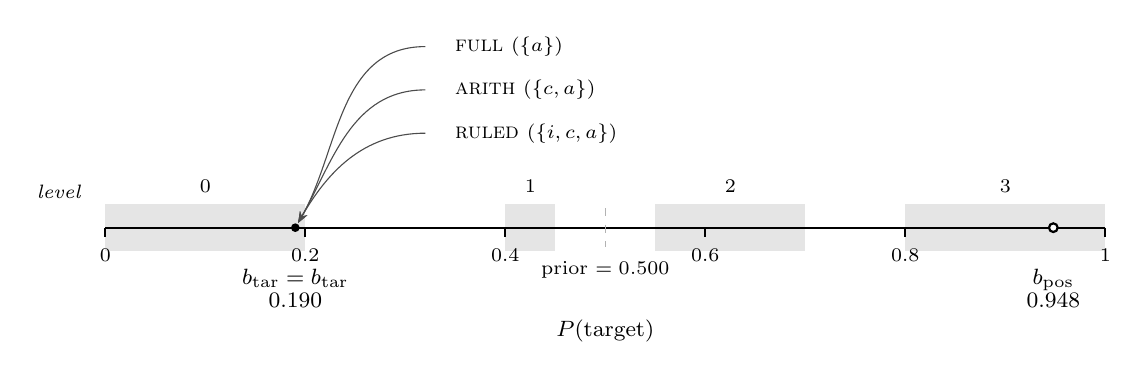
\begin{tikzpicture}[x=12.7cm, y=1cm]
    % --- four response bands, drawn first so everything overlays them.
    %     The three intervals between them are LEFT WHITE on purpose. ---
    \foreach \a/\b in {0.00/0.20, 0.40/0.45, 0.55/0.70, 0.80/1.00}
      \fill[gray!20] (\a,-0.30) rectangle (\b,0.30);
    % band level digits, centered above each band
    \foreach \x/\lab in {0.10/0, 0.425/1, 0.625/2, 0.90/3}
      \node[anchor=south, font=\scriptsize] at (\x,0.32) {\lab};
    \node[anchor=east, font={\scriptsize\itshape}] at (-0.015,0.46) {level};

    % --- the axis, on top of the bands ---
    \draw[thick] (0,0) -- (1,0);
    \foreach \x in {0.0,0.2,0.4,0.6,0.8,1.0}
      \draw[thick] (\x,0) -- (\x,-0.12);
    \foreach \x/\lab in {0.0/0, 0.2/0.2, 0.4/0.4, 0.6/0.6, 0.8/0.8, 1.0/1}
      \node[anchor=north, font=\scriptsize] at (\x,-0.15) {\lab};
    \node[anchor=north, font=\footnotesize] at (0.5,-1.05) {$P(\text{target})$};

    % --- prior pi = 0.500: dashed reference only, no marker, sits in the gap ---
    \draw[gray!60, dashed] (0.5,0.25) -- (0.5,-0.25);
    \node[anchor=north, font=\scriptsize] at (0.5,-0.31) {prior $= 0.500$};

    % --- target b* = q0 = 0.190: FILLED disc (the visual focus) ---
    \node[circle, fill=black, inner sep=0, minimum size=0.11cm] at (0.19,0) {};
    \node[anchor=north, font=\footnotesize, align=center] at (0.19,-0.40)
      {$\bstar = \qz$\\[-1pt]$0.190$};

    % --- silence-blind b_pos = 0.948: OPEN circle (encoding must survive grayscale) ---
    \node[circle, draw=black, thick, fill=white, inner sep=0,
          minimum size=0.11cm] at (0.948,0) {};
    \node[anchor=north, font=\footnotesize, align=center] at (0.948,-0.40)
      {$\bpos$\\[-1pt]$0.948$};

    % --- three transcripts, three operation sets, one target ---
    \foreach \y/\name/\opset in {%
        2.30/{\cond{full}}/{\{a\}},
        1.75/{\cond{arith}}/{\{c,a\}},
        1.20/{\cond{ruled}}/{\{i,c,a\}}} {
      \node[anchor=west, font=\footnotesize] at (0.34,\y)
        {\name~{\scriptsize$(\opset)$}};
      \draw[-{Stealth[length=4pt]}, thin, black!70, shorten >=2pt]
        (0.32,\y) to[out=180, in=60] (0.19,0);
    }
  \end{tikzpicture}
  \caption{%% <ITEM66> Caption text.
  Three transcripts, one target. \cond{full}, \cond{arith}, and
  \cond{ruled} display different channels and require different
  operations, but all three return the same correct belief, so the distance
  between an elicited answer and that belief is comparable across them.}
  \label{fig:schematic}
\end{figure}
\fi %% end FIGURE 1 comment-out (revive with the \iffalse above)

%% =====================================================================
\section{The framework}\label{sec:framework}
%% BUDGET 0.75 pages. THE CONTRIBUTION, and the largest non-example section
%% by design. NOTHING IN THIS SECTION MOVES UNDER PAGE PRESSURE.
%% =====================================================================

%% SETUP paragraph. State |A| = 2 EXPLICITLY: one-dimensionality depends on
%% it, and the word "coordinate" is literal only there. |A| = 2 is
%% load-bearing and must point forward to the one-bin degeneracy in S6 and
%% the limitation in S7.
%% LINEAGE, one clause: the bookbag-and-poker-chip paradigm of Phillips and
%% Edwards, conditioned on a disclosure rule. Costs a clause, buys legitimacy.
%% <ITEM66> Claim text. Read once more in your own voice before submitting.
Two candidates $A=\{a_0,a_1\}$ are under consideration and exactly one is
responsible, with a uniform prior. We take $|A|=2$, and this
one-dimensionality makes this framework truly a "coordinate system", and
it is the source of a structural limitation mentioned in
Section~\ref{sec:blind}. Each of the $N$ analysts runs a binary assay returning \textsc{positive} or
\textsc{negative}. If $a_0$ is responsible, an assay returns \textsc{positive}
with probability $p$; if $a_1$ is responsible, an assay returns \textsc{positive} 
with probability $1-p$. The results are independent given which candidate is responsible. 
We take $1/2 < p < 1$,
so a \textsc{positive} is more consistent with $a_0$ than with $a_1$ and it tilts the reference belief
toward $a_0$. What the observer's transcript shows is controlled by
a \emph{disclosure rule}, and it is this rule that makes our conditions vary: some
display every result, while others only file the $k$ \textsc{positive} reports and leave the
$N-k$ \textsc{negative} reports as absences to be recovered through the value of $N$ and the 
count of filed reports. This is the bookbag-and-poker-chip
paradigm of \citet{phillips1966} conditioned on a disclosure rule. Therefore, the 
transcript displays different channels across different conditions, as seen in
Table~\ref{tab:map}. It is the channel set a transcript exposes
that determines both the operations a correct observer must perform and the
belief it should hold. 

%% REFERENCE BELIEFS -- three displayed numbered equations. L(a) is the
%% likelihood of a positive under candidate a.
%% <ITEM66> Claim text. Read once more in your own voice before submitting.
Write $L(a)$ for the probability that a given analyst's assay returns positive
under candidate $a$, and let $k$ be the number of positives from the $N$
assays. Two beliefs are definable from the transcript alone:
%
\begin{align}
  \bpos(a) &\;\propto\; L(a)^{k}, \label{eq:bpos}\\[2pt]
  \qz(a)   &\;\propto\; L(a)^{k}\,\bigl(1-L(a)\bigr)^{N-k}. \label{eq:qzero}
\end{align}
%
%% One sentence per equation, in this order:
%%  (1) reads the positives as if they were the whole record
%%  (2) treats every absence as a negative finding: the correct posterior, the target
%% <ITEM66> Claim text. Read once more in your own voice before submitting.
Equation~\eqref{eq:bpos} reads the positive filed reports as if they were the
whole record; call it the silence-blind belief $\bpos$. 
Equation~\eqref{eq:qzero} instead scores every absence as a negative finding. Under the disclosure rule,
this is the correct posterior; call it the target $\btar$. These are the two reference beliefs on 
the interval on which the observer's answer is located. 


%% ---------------------------------------------------------------------
%% SHARED TARGET -- the design's asset. The three conditions convey the same N
%% results, so they share the target; no pivot needed once delta is out.
%% Then ONE sentence on exact-rational verification, no floating point.
%% ---------------------------------------------------------------------
%% <ITEM66> Claim text. Read once more in your own voice before submitting.
This design's asset is that the conditions that print the negatives, enumerate
the absences, or leave them to be derived all encode the same information about the $N$
reports. They all return the same target, which makes their comparison valid. 
\\
%% ---------------------------------------------------------------------
%% LEMMA 1 -- ordering. Two-belief version: b_pos strictly above the target
%% in log-odds. This is what licenses the words "between" and "coordinate".
%% Requires |A| = 2 and at least one absence.
%% ---------------------------------------------------------------------
\begin{lemma}[Ordering]\label{lem:order}
Let $|A| = 2$ and $1/2 < p < 1$, and consider a transcript with at least one
absence ($N - k \ge 1$). Then the silence-blind belief places strictly higher
log-odds on $a_0$ than the target does: reading the silence moves belief strictly
below the silence-blind level.
\end{lemma}
\begin{proof}
Let $a_0$ be the candidate with $L(a_0)=p$ and $a_1$ the other, so $L(a_1)=1-p$
and $p>1/2$ gives $L(a_0)>L(a_1)$. Write $\Lambda(b):=\log\frac{b(a_0)}{b(a_1)}$
for the log-odds a belief $b$ places on $a_0$. The two beliefs share the
presence term $k\log\frac{p}{1-p}$ and differ only in how the $N-k$
absences are scored:
\[
  \Lambda(\bpos) = k\log\tfrac{p}{1-p}, \qquad
  \Lambda(\btar) = k\log\tfrac{p}{1-p} + (N-k)\log\tfrac{1-p}{p}.
\]
Because $p>1-p$, $\log\frac{1-p}{p}<0$, so with at least one absence
($N-k\ge1$) every absence strictly lowers the log-odds on $a_0$, so
$\Lambda(\btar)<\Lambda(\bpos)$.
\end{proof}

%% ---------------------------------------------------------------------
%% TABLE 1 -- the map. The paper's most information-dense object.
%% LAYOUT RISK: Table 1 carries S2, S4, and S5 simultaneously.
%% CONTINGENCY: split the operations column into a separate two-column table
%% and leave Table 1 as condition -> channels -> target.
%% ---------------------------------------------------------------------
\begin{table}[t]
  \caption{%% <ITEM66> Caption text.
  The map. Each condition's transcript exposes a different channel set, which
  determines both the operations a correct observer must perform and the
  belief it should hold. Rows 2 through 4 differ in operations yet agree on
  target.}
  \label{tab:map}
  \centering
  \small
  \begin{tabular}{llll}
    \toprule
    condition & channels in transcript & operations required & target \\
    \midrule
    \cond{blind} & positives & aggregate & $\bpos$ \\
    \cond{full}           & positives, printed negatives & aggregate & $\bstar$ \\
    \cond{arith}      & positives, enumerated absences & convert, aggregate & $\bstar$ \\
    \cond{ruled} & positives, derivable absences & identify, convert, aggregate & $\bstar$ \\
    \bottomrule
  \end{tabular}
\end{table}

%% OPERATIONS paragraph. Define the three: identify, convert, aggregate.
%% State the nesting {a} subset {c,a} subset {i,c,a}, which is the
%% ladder Example 2 walks.
%% ONE PRE-EMPTIVE CLAUSE (item 32, avenue 3): why identify is a single
%% operation, namely that once N is stated, noticing that reports are missing
%% and identifying which are missing are the same subtraction. This forecloses
%% the extra-stage reading at the cost of one clause.
%% ONE HONEST SENTENCE in the same place: aggregate is never isolated, since
%% no condition sits below {a}.
%% <ITEM66> Claim text. Read once more in your own voice before submitting.
Three operations appear in Table~\ref{tab:map}. To \emph{identify} is to
determine if reports are absent and how many; if $N$ is present in the transcript,
this boils down to a single subtraction, so noticing the absences and 
counting them are two different parts of one step. To \emph{convert} is to read an absence as a
negative finding. To \emph{aggregate} is to combine the findings into a
posterior. The three conditions sharing a target have the nested required operation
sets $\{a\} \subset \{c,a\} \subset \{i,c,a\}$, which Example~2 investigates.
One honest limit follows: aggregation is never isolated,
because no condition in our design sits below $\{a\}$.

The object we measure is the observer's ability to reason
with evidence that is not explicitly written in the transcript but is derivable 
from understanding its disclosure rule. The reference beliefs give points to compare
the observer's response to: in a condition where the absences are 
derivable, occupancy of $\bpos$ is diagnostic of failing to incorporate the silent
evidence, while occupancy of $\btar$ indicates success in using that evidence to reach
the target posterior.

%% =====================================================================




\section{The instrument}\label{sec:instrument}
%% BUDGET 0.65 pages.
%% =====================================================================

%% SECTION LEAD-IN + ROSTER. Models introduced first, chronologically.
The framework from Section~\ref{sec:framework} provides the interval with
reference beliefs for any
observer that reads such a transcript. We now put real LLM observers on it,
running the conditions of Table~\ref{tab:map} as prompts and plotting each
model's response on the same coordinate.
The seven configurations we initially tested span four model families: 
\texttt{openai/gpt-5.6-sol},
\texttt{z-ai/glm-5.2}, \texttt{deepseek/deepseek-v4-flash-0731}, and
\texttt{meta-llama/llama-3.3-70b-instruct}. Every family except the Llama one
contributes two configurations that differ in reasoning setting and the paired
token budget, which is what the "-high" suffix on a configuration name denotes
(abbreviated "-hi" in Figure~\ref{fig:results} and Figure~\ref{fig:repair}); Appendix~\ref{app:models}
gives the full table.

\subsection{The response scale}

%% RESPONSE SCALE. Four ordinal levels from two enum fields,
%% candidate x two-level confidence.
%% BANDS WERE MEASURED, NOT ASSUMED. Row 1.4, rewritten rev 4:
%%  - measured on BOTH sides; the low side was measured rather than mirrored
%%  - measured edges 0.20 and 0.80
%%  - asymmetry 0.000 at the widest for SIX OF SEVEN configurations on
%%    wording B, which is the wording v2 runs
%%  - llama is the SOLE EXCEPTION (asymmetry 0.1)
%%  - BANNED: "all seven configurations agreed"
%%  - STATED LIMITATION: CAL samples at 0.10 resolution, so the nominal
%%    0.25/0.75 cuts and the alternate 0.20/0.80 edges both fall inside the
%%    measured interval. Invariance across the two is a SAMPLING-RESOLUTION
%%    FACT, not a robustness result, and must be stated as such.
%%  - pre-test population: 32 stimuli x 3 DRAWS x 7, 659/672 usable.
%%    Three draws, not five. Any "five draws throughout" sentence must carve
%%    out the pre-test.
Answers are elicited on two axes, the candidate they think is responsible
and whether they are "Somewhat confident" or "Very confident" in their answer,
giving four ordinal levels. We elicit an ordinal level rather than a
raw probability on purpose: a numerical posterior produced by an LLM
would confound the ability to reason from the evidence with the ability to carry
 out the arithmetic of Bayesian updating, so coarsening the answer into four ordinal levels
  strips out most of the noise of that arithmetic and keeps the signal we really mean
   to measure, whether
the observer moves its belief in the right direction and by how much. 


The probability ranges these four levels occupy were measured, not assumed.
In a calibration pre-test, each configuration is given the stated probability for a candidate
being responsible. With no inference to perform, the LLM responds with its internal mapping
from a numerical probability to either "Very confident" or "Somewhat confident" (Appendix~\ref{app:calib}).
For six of the
seven configurations, the switch that separates the two ordinal levels is at $0.20$ on the low side
 and $0.80$ on the
high side, with \texttt{llama} being the lone exception.
A model is very
confident in a candidate once its probability clears $0.80$, very confident
in the other candidate below $0.20$, and merely somewhat confident closer to even
odds.

%% THE BAND GAPS ARE LOAD-BEARING. The response scale has deliberate gaps
%% between the four levels; every cell is built so both b_pos and the target
%% land inside a band, not a gap. The 0.45-0.55 gap straddles the 0.5 prior,
%% which Example 1's occupancy split uses.
The four levels sit in measured bands with deliberate gaps between them: level
$0$ is $[0,0.20]$, level $1$ is $[0.40,0.45]$, level $2$ is $[0.55,0.70]$, and
level $3$ is $[0.80,1]$ (Appendix~\ref{app:calib}). Every cell is built
so that both the silence-blind belief and the target land inside a band rather
than one of these gaps, giving each a definite level to score against.

%% DESIGN CONSTRAINTS, four clauses:
%%  - every cell asserts level(b_pos) != level(target) at build time.
%%    Verified fourteen for fourteen.
%%  - prompts never use silence vocabulary, enforced by a forbidden-word
%%    list at build.
%%  - every stimulus appears in both label orderings.
%%  - count-control cells invert the correct level, so a fixed
%%    high-confidence responder is separable from a competent one.
Four constraints are enforced at build time. Every cell is designed so that the
silence-blind belief and the target fall in different levels, which holds in
all fourteen cells.
A build-time forbidden-word list bans silence vocabulary together with Bayesian
and computational vocabulary, so no cues are given in the prompt for what operation it is testing.
Every stimulus is tested with both label orderings. Count-control cells invert the correct
level, so a configuration that always answers high-confidence is separable from
a competent one. These controls are intended to distinguish evidence-sensitive inference 
from heuristics based on the number of positive reports. Appendix~\ref{app:prompts} 
reproduces the prompts, the response
schema, and one rendered stimulus per condition.

\subsection{The competence gate}

Before reading any configuration against the coordinate, we check that it is able to 
read the record at all. A competence gate is built on two conditions from the same 
underlying record. In the
printed-negatives condition (\cond{full}), every result, positive and negative,
is displayed and completeness is asserted, so reaching the correct answer is a
matter of aggregation, while in the derivable-absences condition (\cond{ruled}),
only the positive reports appear, and the negatives must be inferred from the
stated analyst count and filing rule. A configuration that fails the
printed-negatives condition is excluded, because a configuration that fails
both conditions is a floor effect rather than a silence result.

%% STATISTICS.
%%   s1 = |l_obs - l_cor|
%%   s2 = l_obs - l_cor  (positive = under-weighted toward the target)
%%   l_cor = level(target(C)) read off Table 1.
To measure where a model lands on the coordinate, we need a distance in
levels. We now define the statistics that report it.
We report $s_1 = |\lobs - \lcor|$ and the signed $s_2 = \lobs - \lcor$, with
positive values meaning under-weighting toward the target, where $\lobs$ is the
level of observer reports and $\lcor$ is the level of the target read off
Table~\ref{tab:map}. With this, five of seven configurations are admitted, at mean $s_1$
on the printed-negatives condition of $0.200$, $0.421$,
$0.457$, $0.752$ and $0.764$ levels; the two excluded sit at $1.609$
(\texttt{deepseek}) and $1.800$ (\texttt{llama}). A mean $s_1$ above one means that, on average, the
answer lands more than a full level from the target, so the gate sets these two aside. 
All results in the next two sections are therefore reported only for those five: 
the configurations that demonstrate a baseline ability to perform inference 
with all evidence printed. The results below should 
then be read as characterizing silence-reading behavior among models with 
this baseline inference ability and not all LLMs generally.

%% END PARAGRAPH: llama consistency + campaign totals + pre-registration.
%% llama is the exception in FOUR INDEPENDENT PLACES -- W1 reachability,
%% W1 wording stability, W1 low-high asymmetry, and the competence
%% gate -- plus P4 on D1-D3. CONSISTENCY RESULT, not five separate caveats.
%% CAMPAIGN (delta=0 subset): 5,808 usable of 5,950 attempted, 5 draws/stimulus.
%%   = 2,894 + 959 + 1,955 usable / 2,940 + 980 + 2,030 attempted (the three
%%   delta=0 arms; the two delta=0.3 arms 620/630 + 623/630 are removed).
%%   The W1 pre-test's 659/672 sits OUTSIDE that total, 3 draws, different set.
%% PRE-REGISTRATION: R4 APPLIES HARD; scoring deferred to S6.
The campaign
holds $5{,}808$ usable draws of $5{,}950$ attempted, at five draws per stimulus;
the pre-test described above contributes a further $659$ of $672$ on a separate
stimulus set at three draws per stimulus.



%% =====================================================================
\section{Example 1: which direction does the error run?}\label{sec:ex1}
%% BUDGET 0.60 pages.
%% OPEN ITEM: headline ordering. Toggle \anchorleadtrue / \anchorleadfalse
%% in the preamble to order \ParaAnchor (occupancy + extremity) against
%% \ParaTallies (the D-cell tallies). The prior-crossing support was cut
%% 2026-08-27, so \ParaAnchor now rests on the occupancy result and the
%% extremity refutation.
%%
%% NOTE the dependency: S4's arbitration sentence locates the over-updating
%% regime using S5's result. Either order them accordingly or state the
%% dependency explicitly.
%% =====================================================================

%% P1 -- THE DISAGREEMENT (rewritten 2026-08-21).
%%  - Imran et al.: PRE-TRAINED models update less than Bayes requires,
%%    shortfall shrinking as models scale; measured over token log-probs on
%%    pre-trained checkpoints. Gradient < 1 for EVERY model tested.
%%  - BayesBench: BOTH DIRECTIONS on INSTRUCTION-TUNED models, SPLIT BY
%%    SCALE. Smaller models stay near the middle, larger models push toward
%%    the extremes. MAE at theta=0.5 rises 8.3 (LLaMA-3B) -> 36.7 (Qwen-32B)
%%    -> 34.2 (LLaMA-70B).
%%  - DO NOT WRITE "BayesBench reports over-confidence". That was the
%%    record's error, corrected at item 36.
%%  - The populations DO NOT OVERLAP and that is load-bearing.
%%  - Construct name: conservatism, after Edwards.
Whether language models update too little or too much is contested, and the two
closest anchors disagree, on the populations that do not overlap.
\citet{imran2025} report that pre-trained-only checkpoints update less than
a correct Bayesian update would, with the shortfall shrinking as models scale, measured over
token log-probabilities. They describe the shortfall as unexplained and
note that it may be a result of how improbable their evidence strings are, so we take
the direction from them and not a mechanism. \citet{bayesbench2026} evaluate
instruction-tuned models across turns and report that smaller models stay near 
the middle of the interval, while larger ones can push toward the extremes when the evidence is
skewed. Under-use relative to Bayes has been called conservatism since
\citet{edwards1968}.
%% <ITEM66> replaces two sentences (audit item 2); the removed pair wrongly said
%% both anchors score against a model-supplied reference -- BayesBench has
%% closed-form Bayesian references in two of its four environments.
Imran et al.'s expected update is elicited from the model, read from
its own token probabilities, and where a closed-form reference is available
elsewhere, it is computed from evidence the observer can see.
\citet{gupta2025} show that updates track the Bayesian
posterior closely when enough of that evidence has accumulated in the model's
context. Our target is computed from the disclosure rule,
so the question here is not whether a belief moves correctly on
what the transcript displays but whether it moves on what it
withholds.

%% P2 -- THE DISCLOSURE. Plain, unburied, one sentence.
%% BOTH ANCHORS WERE SELECTED AFTER THE DATA EXISTED. The campaign was
%% registered; the literature engagement was not.
%% <ITEM66> Claim text. Read once more in your own voice before submitting.


%% P3 -- THE SETUP IN FRAMEWORK TERMS.
%% Two channel sets, {positives, printed negatives} and {positives, derivable
%% absences}, returning different operation sets but THE SAME TARGET
%% (same information).
%% EXPRESSIBILITY LEDGER (row 2.4), ships with every one-sidedness statement:
%% b* < b_pos in every cell; l_cor = 0 in 11 of 14 cells; so over-weighting is
%% only EXPRESSIBLE where l_cor >= 1, which is cells D1-D3.
%% STATE THE DENOMINATOR HONESTLY AND UP FRONT.
The comparison uses two channel sets, printed negatives against derivable
absences, which require different operations but share a target. 
Because the target lies below the silence-blind
belief in every cell, an answer that under-weights the absence of a report stays high, above
the target, while one that over-weights it falls below. The first eleven cells have a
target on level 0 (Appendix~\ref{app:cells}), so nothing lies
below it and over-weighting is structurally inexpressible. We therefore designed three cells, 
D1--D3, with the target one level up specifically so that an answer can fall on either
side of it. These three cells are where under-weighting and over-weighting are both
expressible, and the direction-of-error result is measured on them.

%% ---------------------------------------------------------------------
%% The two result paragraphs are defined as macros so the two candidate
%% orderings cannot drift apart. Flip \anchorleadtrue in the preamble.
%% ---------------------------------------------------------------------

%% P4 -- THE RESULT AND THE CONTROL (restructured, item 30 part 1).
%% THE ARMS ARE NOT SYMMETRIC EVIDENCE. The gate selects on FULL, and V-24-2
%% made FULL a claim-carrying arm. THE 0/300 MUST NOT BE POOLED.
%%   RESULT: RULED on D-cells runs 47-0 toward under-weighting across
%%     the five gated configurations. 150 attempted, 150 usable, zero
%%     failures. Attempted is the stronger denominator and costs nothing.
%%     Gate on FULL, outcome on RULED, so this arm is unselected.
%%   CONTROL: FULL runs 9-0, same 150 attempted. Direction persists under an
%%     easier channel set among configurations chosen for accuracy there.
%%     All five FULL over-reads across the full roster come from llama and
%%     deepseek, exactly the two the gate excluded, so this arm CANNOT be
%%     independent corroboration.
%% SIGNIFICANCE AT THE REGISTERED GRAIN (R5, item 41): the cell is the unit,
%% mirrors and draws pooled to one modal level.
%%   Two-sided exact sign test over the 15 config-by-cell units:
%%     RULED 8-0, p = 0.008 ; FULL 5-0, p = 0.063
%%   The result arm survives at the registered grain; the control does not
%%   reach significance and does not need to.
%%   The remaining 7 units carry no displaced mass and are UNDEFINED rather
%%   than failed.
%% BANNED: p ~ 0.004 (2 x 0.5^9 at draw level; contradicts the item-78
%% sentence that the paper assumes no independence across draws).
%% Also BANNED here: the 176 and 206 denominators.
\newcommand{\ParaTallies}{%
\textbf{The error runs one way.} Out of $150$ draws spread across the three cells and five admitted configurations, 
$47$ missed the target posterior, and every one of those $47$
errors under-weights the silence while not a single draw over-weights it
(Figure~\ref{fig:results}a). The competence gate admits configurations by their performance on the
printed-negatives condition and not on the derivable-absences one, so the arm
that carries the result played no part in the selection.
At the unit of analysis, a configuration's modal answer on a cell, 
eight of the fifteen configuration-by-cell
units are displaced toward under-weighting and none toward over-weighting
(two-sided exact sign test, $p = 0.008$); the remaining seven carry no displaced
mass. This direction persists in the
printed-negatives condition: $9$ to $0$ on the same $150$ draws, five
of fifteen units displaced, $p = 0.063$. Among errors that the instrument 
can express in these cells, the admitted configurations display a strong directional 
tendency to under-weight the silence rather than over-weight it.
}

%% P5 -- OCCUPANCY + THE FOURTH KILLED ALTERNATIVE.
%% The b_pos-anchoring / prior-crossing claim (old row 2.5, the 8/91 .. 17/52
%% numerators) was CUT 2026-08-27 as weak -- see the ledger. What remains here is
%% the occupancy result (now Figure 2b) and the extremity refutation.
%% Blind-point occupancy FALLS IN NONE OF FIVE and rises in four
%%   (0->4.6, 12.4->30.6, 6.4->77.1, 0.7->6.4; sol-high 0->0 at ceiling).
%%   BANNED: "5/5" occupancy.
%% ONE CLAUSE ON WELL-DEFINEDNESS (row 2.6): the uniform prior at 0.5 falls
%%   inside the 0.45-0.55 band gap, which straddles it exactly, so levels 0
%%   and 1 lie wholly below and 2 and 3 wholly above, with no level ambiguous.
%% THE FOURTH KILLED ALTERNATIVE (row 2.13, G2.4 closed). One clause, and it
%%   answers the strongest anchor-derived objection to claim 2:
%%   BayesBench's triage result is that models sharpen the extremes and
%%   collapse the middle two. On this scale levels 1 and 2 ARE the middle two,
%%   so extremity predicts level-1 draws moving to level 0. Observed: they
%%   move to LEVEL 2. Not a weaker version of extremity, the OPPOSITE
%%   direction, landing on the interior anchor the b_pos account names in
%%   advance.
%%   Of the 47 displaced RULED draws: 44 at level 2 = level(b_pos), 3 at
%%   level 3, 0 at level 0. Endpoint mass 3 of 150 attempted, 2.0%.
%%   Level 2 outnumbers level 3 in ALL THREE configurations with displaced
%%   mass to test: glm-high 5 vs 1, deepseek-high 11 vs 0, glm 28 vs 2. The
%%   sol family produces none, so undefined rather than failed.
%%   FULL: 9 at level 2, 0 at level 3.
%% REBUTTAL ON FILE, if a referee raises prior miscalibration (Gupta et al.
%% 2025). Their account predicts error mass at the model's OWN fixed internal
%% bias, which would put it at the SAME level in every cell. Our at-l_pos mass
%% tracks l_pos as l_pos moves: level 2 in the B and D cells, level 3 in the
%% A and C cells. See glm's RULED row in paper/audit/geometry_by_distance.md
%% (28 and 24 at level 2 for dist=1 and dist=2; 56 at level 3 for dist=3).
%% A constant model-internal prior cannot produce a location that tracks a
%% computed quantity. NOT in live text; page budget.
\newcommand{\ParaAnchor}{%
\textbf{Occupancy.} We also ask how often belief resides on the silence-blind belief,
and whether that changes based on the channels in the transcript.
Occupancy of that level, the fraction
of draws that land on it, is measured for the five admitted configurations
over all cells, under both the printed-negatives and derivable-absences conditions
(Figure~\ref{fig:results}b). Occupancy of the silence-blind level either
rises or stays the same when the negatives must be inferred rather than read,
so the evaluated configurations settle on the silence-blind belief more often when the 
silence has to be recovered.

%% Figure 2 serves the tallies and occupancy paragraphs above; the extremity
%% paragraph below is a separate point (float moved here 2026-08-27).
\begin{figure}[t]
  \centering
  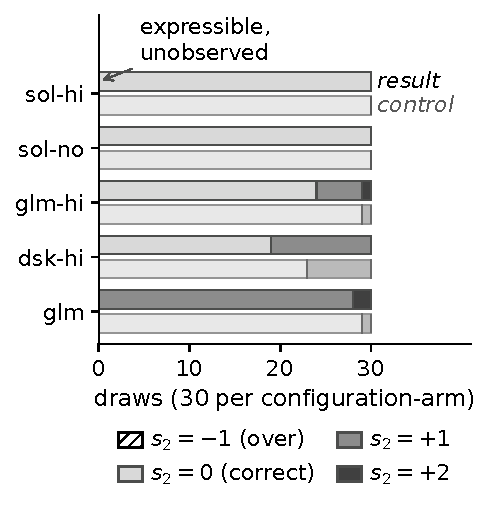
\includegraphics[width=0.48\textwidth]{figures/results_signed_error.pdf}\hfill
  %% Panel (b): silence-blind-level occupancy, FULL vs RULED (make_occupancy.py).
  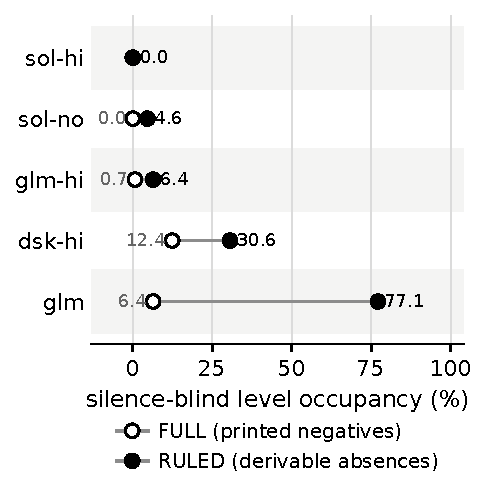
\includegraphics[width=0.48\textwidth]{figures/results_occupancy.pdf}%
  \caption{%% <ITEM66> Caption text.
  \textbf{(a)} Signed displacement $s_2$ on the three cells where over-weighting
  is expressible, five admitted configurations, $150$ attempted draws per arm;
  the result arm is derivable-absences, the control (gate-selected) is
  printed-negatives. The $s_2 = -1$ (over-weighted) segment has zero width in
  every bar. \textbf{(b)} Occupancy of the silence-blind
  level, the percent of draws landing exactly on it, under the
  printed-negatives condition (open marker) and the derivable-absences one
  (filled), for the five admitted configurations over all 14 cells.
  Occupancy rises in four of the five and falls in
  none, reaching $77.1$ percent for \texttt{glm}; \texttt{sol-hi} sits at zero in
  both. Configurations are abbreviated (\texttt{dsk}${=}$deepseek).}
  \label{fig:results}
\end{figure}

An ordinal extremity effect predicts mass piling at the endpoints. However, 
of the $47$ displaced
draws, $44$ land at the level of the silence-blind belief, which is not an
endpoint, $3$ land at the top level, and none at the bottom, so total endpoint
mass is $3$ in $150$ draws. In all configurations with displaced mass to test,
mass at the internal silence-blind level outnumbers mass at the endpoint.%
}

%% ---- render in the selected order ----
\ifanchorlead
  \ParaAnchor

  \ParaTallies
\else
  \ParaTallies

  \ParaAnchor
\fi

%% P5b -- REQUIRED (row 2.12). The answer to "your roster is too small to
%% produce the over-direction": the over-direction IS recoverable on this
%% instrument with these models, via the ARITH over-reads. Since BayesBench
%% makes over-updating a large-model behaviour, S4 MUST contain this.
%% This is also where the S5 dependency is discharged.
%% <ITEM66> Claim text. Read once more in your own voice before submitting.
The one-sidedness here is a property of the information in the transcript
and not of the instrument. In Section~\ref{sec:ex2}, over-weighting is seen
with the same models, but with different channel sets. The objection that our 
roster is too small to produce it becomes the observation
that our instrument sees it only where the transcript enumerates the absences.


%% =====================================================================
\section{Example 2: identification or interpretation?}\label{sec:ex2}
%% BUDGET 0.60 pages.
%% CUT, NOT DEMOTED (item 32): the cross-regime contrast is OUT. It brushed
%% three closed avenues at once and is 2 of 3 once gated. Do not reinstate.
%% =====================================================================

%% P1 -- THE QUESTION. When a system fails to use silence, is it failing to
%% NOTICE the absences or failing to INTERPRET them? In general the two are
%% confounded.
When an observer fails to reason on the absences, it may be failing to notice them or
failing to understand what they mean in context. In general,
 these two are confounded,
because a task that makes absences easier to identify usually also makes them
easier to interpret.

%% P2 -- WHY THE LADDER EXISTS. Table 1 rows 4, 3, and 2 have strictly nested
%% operation sets {i,c,a} superset {c,a} superset {a} and, by shared information,
%% ONE SHARED TARGET. Each rung deletes exactly one operation, and the channel
%% change is the mechanism of deletion. No ad-hoc design yields this; it falls
%% out of the map.
Table~\ref{tab:map} separates them without a new task. Its three shared-target
conditions (\cond{full}, \cond{arith}, and \cond{ruled}) have
strictly nested operation sets, so moving up the ladder deletes
exactly one operation and changes nothing else, and the deletion is done simply
by changing the channels in the transcript. This does not have to be designed
in; it falls out of the map.

%% CEILING GUARD. A written decision criterion (0.15-bin gap). The empty gap is
%% the load-bearing, verifiable fact.
To separate the failure to identify the absences from the failure to interpret
them, we compare a configuration's answers when the absences must be inferred
(the derivable-absences condition) against its answers when they are listed out
(the enumerated condition). 
Because both conditions state the same filing rule as seen in Appendix~\ref{app:prompts},
the only additional operation 
required with derivable-absences is to identify the $N-k$ absent reports from the stated 
analyst count. Whatever accuracy enumerating the absences recovers is what the
configuration could not identify on its own. 

However, that comparison only means something
for a configuration that has trouble reading silence in the first place. Some
configurations do not: they handle the condition where the absences must be
inferred about as well as the condition where every result is printed, so they carry minimal
difficulty in identifying and interpreting silence. Trying to quantify how much the 
enumeration of absences helps these configurations reason would be measuring 
repair where there was nothing to repair.

We separate these configurations with a written decision criterion. A configuration's difficulty with silence is the gap
between its error when the absences must be inferred and its error when every
result is printed, $s_{1,\mathrm{RULED}} - s_{1,\mathrm{FULL}}$. A configuration
for which that gap is below $0.15$ levels is declared \emph{at ceiling} and set
aside as uninformative for identification localization. These
configurations are at the ceiling of silence-reading ability, and this section
asks about configurations with a genuine deficit in identifying absences. 
The threshold falls in an empty gap (Table~\ref{tab:ceiling}).

\begin{table}[H]
  \caption{Silence-reading difficulty per admitted configuration: cell-weighted
  mean $s_1$ on the derivable-absences and printed-negatives conditions and their
  difference, over cells. The $0.15$-level threshold
  falls in an empty gap. \texttt{sol-high} and \texttt{glm-high} sit well below it
  and near zero (\texttt{sol-high} is negative, scoring better when the absences
  must be inferred than when they are printed), so these two read silence with
  essentially no difficulty; the other three have a visible deficit, and the
  localization comparison is only valid for them.}
  \label{tab:ceiling}
  \centering
  \small
  \begin{tabular}{lrrr}
    \toprule
    configuration & $s_{1,\mathrm{FULL}}$ & $s_{1,\mathrm{RULED}}$ &
      $s_{1,\mathrm{RULED}} - s_{1,\mathrm{FULL}}$ \\
    \midrule
    \texttt{sol-none}      & $0.431$ & $0.762$ & $0.331$ \\
    \texttt{deepseek-high} & $0.758$ & $1.020$ & $0.261$ \\
    \texttt{glm}           & $0.764$ & $2.243$ & $1.479$ \\
    \midrule
    \texttt{sol-high}$^{\ast}$ & $0.200$ & $0.114$ & $-0.086$ \\
    \texttt{glm-high}$^{\ast}$ & $0.457$ & $0.486$ & $0.029$ \\
    \bottomrule
  \end{tabular}\\[2pt]
  {\footnotesize $^{\ast}$ at ceiling
  ($s_{1,\mathrm{RULED}} - s_{1,\mathrm{FULL}} < 0.15$ levels).}
\end{table}



%% P4 -- THE RESULT, HEADLINE FIRST. Settled 2026-08-21: the headline is the
%% RISING INTERIOR MASS, a universal over the claim population with no
%% fraction to defend.
%%   Blind-point residence collapses for all three non-ceiling gated
%%     configurations: 4.6->0.0, 30.6->12.9, 77.1->50.0. The absences WERE
%%     going unnoticed.
%%   But interior mass RISES IN EVERY ONE OF THEM: 65.4->66.9, 28.4->42.4,
%%     17.1->27.9. The freed answers land short of target.
%%   IDENTIFICATION IS REPAIRED; CONVERSION IS NOT.
%%   glm-high's occupancy RISES 6.4->10.7 and is reported; it sits outside
%%     the population by the registered 0.15-bin ceiling guard.
\textbf{Identification is repaired.} Deleting the identification step frees answers from the silence-blind belief.
Moving from the derivable-absences condition to the enumerated one, occupancy of
that belief collapses in every deficit configuration, from $4.6$ to $0.0$, from
$30.6$ to $12.9$, and from $77.1$ to $50.0$ percent of draws (Figure~\ref{fig:residence}): the absences were
going unnoticed, so enumerating them helped the configuration realize there were silences 
in the first place. We report that for the two ceiling configurations,
\texttt{glm-high} moves the other way, $6.4$ to $10.7$, and \texttt{sol-high}
has no occupancy to lose. Neither follows the pattern from the deficit configurations, as
they have no genuine deficit to repair in the first place. 

\textbf{Interpretation is not.} The answers freed from the silence-blind belief 
do not arrive at the target. Interior mass, the
mass strictly between the silence-blind belief and the target posterior, rises in
every deficit configuration as the step comes out, from $85.0$ to $87.0$, $36.5$
to $54.1$, and $21.8$ to $35.5$ percent on the cells that can express it, with
D1--D3 dropped since these cells have the target and the
silence-blind belief adjacent to each other, so no level lies between them
(Figure~\ref{fig:interior}). Interior mass rises for all five admitted
configurations, but the two ceiling configurations are set aside since we
established that they are uninformative for understanding the split in silence-reading. 

\begin{figure}[H]
  \centering
  \begin{subfigure}[t]{0.49\textwidth}
    \centering
    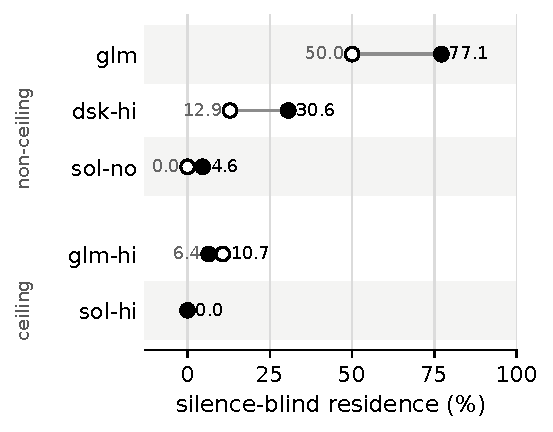
\includegraphics[width=\textwidth]{figures/results_residence.pdf}
    \caption{Occupancy of the silence-blind belief, over cells. It collapses for the three deficit configurations; the two ceiling
    configurations do not follow, with \texttt{glm-hi} rising instead.}
    \label{fig:residence}
  \end{subfigure}\hfill
  \begin{subfigure}[t]{0.49\textwidth}
    \centering
    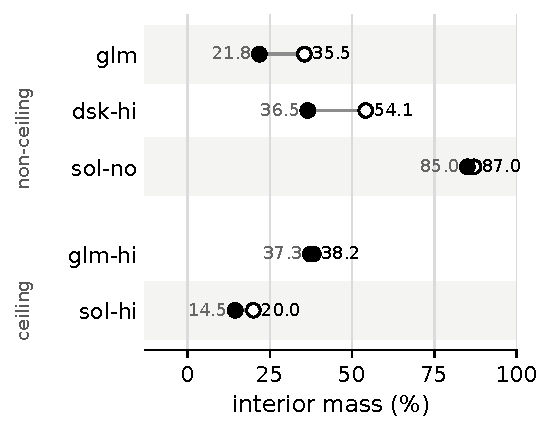
\includegraphics[width=\textwidth]{figures/results_interior.pdf}
    \caption{Interior mass, on the cells that can express it (D1--D3
    excluded, where target and silence-blind belief are adjacent). It rises for
    all five, but the two ceiling configurations are set aside.}
    \label{fig:interior}
  \end{subfigure}
  \caption{Identification is repaired; interpretation is not. Moving from the
  derivable-absences condition (\textsc{ruled}) to the enumerated one
  (\textsc{arith}); filled marker \textsc{ruled}, open marker
  \textsc{arith}, rows grouped by the ceiling guard. \textbf{(a)} occupancy of the
  silence-blind belief collapses, so the absences were going unnoticed;
  \textbf{(b)} the freed mass rises into the interior rather than reaching the
  target (\texttt{dsk}${=}$deepseek).}
  \label{fig:repair}
\end{figure}

Identification is the one operation the derivable-absences
condition needs that the enumerated one does not, so the collapse in occupancy of
the silence-blind belief is evidence that enumerating the absences for the evaluated
configuration improves its ability to recognize that the silences hold some evidential
significance. However, the increase in interior mass is 
evidence that identifying the absences for the configuration is not enough to push it
all the way to the correct answer.

%% P8 -- THE BRIDGE BACK TO S4. Row 4.11, one of the three new assets:
%% over-reading appears once absences are ENUMERATED.
%%   2 over-reads in 150 expressible gated draws in ARITH
%%     (deepseek-high 1/30, glm 1/30) against 0 of 300 in the
%%     non-enumerated arms.
%%   And the two configurations are exactly the two with the largest repairs.
%%   OVER-DIRECTION APPEARS ONLY IN THE ENUMERATED CHANNEL (existence, not a
%%   rate at 2/150). This is the shared spine of S4 and S5.
%% <ITEM66> Claim text. Read once more in your own voice before submitting.
The two halves meet here. Once the absences are enumerated, over-reading appears:
two over-reads in $150$ expressible admitted
draws on the enumerated condition, against none in $300$ on the two conditions
that do not enumerate, and the two configurations producing them are exactly the
two with the largest repairs. So the appearance of over-reading silence is a
property of the channel set.

%% THE ANCHOR (re-anchored to RQ4, 2026-08-28). CROWN-QA is CROSS-METHOD
%% RECOVERY of the identification/interpretation split, the section's thesis.
%%   RQ4 (their Table 7): wrong closure judgments most often first diverge in
%%   the evidence-coverage field (45-72% across 3 models), NOT the final
%%   Boolean -- so the failure is interpretive, upstream of the decision.
%%   We reach the same locus by deleting operations: enumeration repairs
%%   identification, belief still lands short -> interpretation is the residue.
%% Positioning: they hold question+facts fixed and vary query-relative coverage
%%   (does absence license a negative at all); we hold the target fixed and
%%   vary which operations the transcript requires (how far belief should move).
%% <ITEM66> Claim text. Read once more in your own voice before submitting.
This localization is also recovered by a different method in \citet{crownqa2026}.
Decomposing the closure judgment with structured certificates, they find that
reasoning most often first diverges in how the model understands what
the evidence covers. 
We reach a compatible split by removing required operations to see that while
enumeration repairs identification, the belief still lands short of the target. 
The residual failure is interpretive in both cases. 
They hold the question and observed facts fixed and vary how much the
evidence covers what the question asks, asking whether an absence justifies a
negative answer at all, while we hold
the target fixed and vary which operations the transcript requires to read the absences, asking how
far belief should move.

%% =====================================================================
\section{Limitations and future directions}\label{sec:blind}
%% BUDGET ~0.4 pages. Three structural limits (pairs fused by the geometry), then
%% a closing future-directions paragraph. Roster/setting bullets + related-work
%% paragraphs CUT 2026-08-29 per Ali. Characterizations TYPED BY ALI (item 66).
%% =====================================================================

%% LIMITATIONS -- bulleted. Three structural (pairs fused by the geometry) + two
%% scope. |A|=2 is ONE bullet; single-round static is ONE bullet. Count-vs-weight
%% bullet (nats/KL, foreign to the ordinal frame; definitional not a limit) CUT
%% 2026-08-29 per Ali.
%% Numbers: eps0 ~50-60x (5.7); band 1 = 0.40-0.45, gaps 0.20/0.10 (5.8);
%%   |A|=2 one-bin (G4.5).
%% <ITEM66> Claim text. Read once more in your own voice before submitting.
The instrument as designed does have its limitations:
\begin{itemize}
\itemsep0em
  \item \textbf{Isolation against expressibility.} Coarsening each answer to one
    of four ordinal levels is what lets us read the direction and magnitude of a
    model's update without confounding it with its ability to do Bayesian arithmetic,
    but that same coarseness leaves only a small, finite set of
    $(\lpos, \lcor)$ configurations a cell can express, a limit the continuous
    framework does not have. Over-weighting is only expressible when the target
    posterior is not at an endpoint, which is only three out of fourteen cells. 
    This is why the direction test of Figure~\ref{fig:results} rests entirely on 
    just D1--D3, and
    in those same cells, the target and the silence-blind belief occupy adjacent
    levels, leaving no level between them, which is why D1--D3 are dropped from the
    interior-mass panel, Figure~\ref{fig:interior}. The two pull against each
    other: a coarser scale isolates the reasoning signal more cleanly but
    expresses fewer configurations, and a finer one expresses more but lets the
    arithmetic confound the silence-reading we are trying to measure.
  \item \textbf{Over-read against under-read visibility.} 
    For cells D1--D3, $\lcor$ = 1, which sits in $[0.40,0.45]$, the narrowest 
    band in the instrument. It has a gap of $0.20$ below it and $0.10$ above, so
    registering an over-read takes roughly twice the excursion an under-read does.
  \item \textbf{Resolution against candidate count.} With two candidates, the
    silence-blind belief is at least $0.5$ by construction, so it will only ever
    occupy the top two levels. In the cells carrying Section~\ref{sec:ex1}'s
    result, the intermediate region is empty outright, so the $47$--$0$ test lives
    on a one-level span, which follows from fixing $|A| = 2$.
\end{itemize}

%% FUTURE DIRECTIONS -- each limit -> a way to stress/extend the instrument.
%% #1 (isolation/expressibility) + #3 (|A|=2) share the 'richer coordinate'
%% repair; #2 (visibility) -> symmetric bands. Stay in the closed-form setting.
%% <ITEM66> Claim text. Read once more in your own voice before submitting.
Each of these limitations is also a direction for improving the instrument. The first and
third share a repair, a richer coordinate system built off the existing framework:
adding ordinal levels or moving
beyond two candidates would increase the number of belief configurations the current scale
cannot structurally express and make it easier to design cells for testing the way the observer 
can reside relative to the reference beliefs.
The open question is how far the scale can be refined before the arithmetic confound
that the coarse scale excluded returns. The second calls
for a narrower fix: bands placed symmetrically about the target posterior would let an
over-read and an under-read of the same size register equally, removing the
advantage the scale currently gives to under-reading. None of these requires
leaving the closed-form setting that makes the reference beliefs computable to begin with.

%% =====================================================================
%% REPRODUCTION STATEMENT. Cite frozen-outputs commit 9ade4d4.
%% Standing risk 2: FOUR ANALYSIS SCRIPTS CARRY HARDCODED ABSOLUTE PATHS and
%% a reviewer trying the repo hits it immediately. Decide before submitting
%% whether to fix them or to say nothing about running the code on another
%% machine.
%% Standing risk 1: public repo against permanently unknown blind status.
%% =====================================================================
%% <ITEM66> Claim text. Read once more in your own voice before submitting.
%% ADMIN, OPEN. Two things to verify before submitting:
%%   1. Confirm commit 9ade4d4 exists, is pushed, and is reachable publicly.
%%   2. Four analysis scripts carry hardcoded absolute paths (standing risk 2).
%%      Either fix them or do not claim the code runs on another machine. The
%%      sentence below deliberately says "available at", not "reproducible".
\paragraph{Reproduction.} Stimuli, draw records, and analysis scripts are
available at \url{https://github.com/akhan531/Control-On-LLMs}, commit
\texttt{9ade4d4}.

%% <ITEM66> acknowledgments draft; final wording is Ali's.
\section*{Acknowledgments}
This work was supported by the Rutgers Summer Undergraduate Research Fellowship
(SURF) program. The author thanks Dr.~Laurent Burlion for his guidance and
supervision.

%% =====================================================================
%%  BIBLIOGRAPHY
%%  Inline thebibliography, per the chosen file structure.
%%
%%  STATUS FLAGS FROM citation_ledger.md. Anything marked NOT VERIFIED must
%%  be resolved against a primary source before submission. An invented
%%  author list is worse than a missing citation.
%%
%%    VERIFIED : depunder2026, depunder2024, crownqa2026, imran2025,
%%               bayesbench2026
%%    PARTIAL  : eo2026, choi2025, saa2026, absencebench2025, razniewski2024
%%    UNRESOLVED / TO RESOLVE : li2025, zhou2025, zhang2025
%%
%%  ACTION LIST STILL OPEN (citation_ledger):
%%    - G4.7: read Zhang et al. arXiv:2512.18489 (discounted Bayesian
%%      filters). THE ONLY UNREAD ITEM THAT COULD COLLIDE WITH TABLE 1'S
%%      FOURTH OPERATION. If it collides, S2's discount row needs a sentence.
%%    - Resolve eo2026, li2025, zhou2025 to full detail. These carry the
%%      prompting pre-emption and are currently THE WEAKEST BLOCK IN THE
%%      SUBMISSION.
%%    - Item 53: final light related-work pass, scheduled 2026-08-25,
%%      including a version check on BayesBench and CROWN-QA. HARD DATE.
%% =====================================================================
\bibliographystyle{plainnat}
%% DROPPED 2026-08-23. Five entries removed:
%%   eo2026, saa2026  -- cited in the body but bibliographically UNRESOLVABLE.
%%     Neither the title nor the anthology id returns a match. Per the ledger's
%%     own rule (bracket keys expire; resolve against primary sources), an
%%     invented author list is worse than a missing citation. The two sentences
%%     that carried them survive on their remaining citations. RESTORE if you
%%     can resolve them against a primary source.
%%   li2025, zhou2025 -- unresolved AND cited nowhere in the body.
%%   zhang2025        -- bibliographically confirmed via BayesBench's reference
%%     list (Jensen Zhang, Jing Yang, Keze Wang, arXiv:2512.18489, Dec 2025),
%%     but still UNREAD (G4.7) and cited nowhere. Characterizing it from a
%%     secondary source would violate the ledger rule. Read it, then add it
%%     with a citation in the discount row of Section 2.
\begin{thebibliography}{99}

\bibitem[Edwards(1968)]{edwards1968}
W.~Edwards.
\newblock Conservatism in human information processing.
\newblock In B.~Kleinmuntz, editor, \emph{Formal Representation of Human
  Judgment}. Wiley, 1968.
%% Cite the 1968 original, note the 1982 reprint, and use ONE form
%% consistently throughout.

\bibitem[Gupta et al.(2025)]{gupta2025}
R.~Gupta, R.~Corona, J.~Ge, E.~Wang, D.~Klein, T.~Darrell, and D.~M. Chan.
\newblock Enough coin flips can make LLMs act Bayesian.
\newblock In \emph{Proceedings of the 63rd Annual Meeting of the Association
  for Computational Linguistics (Volume 1: Long Papers)}, pages 7634--7655,
  2025. arXiv:2503.04722.
%% VERIFIED, read in full 2026-08-25. Load-bearing: updates track Bayes on
%% PRESENT evidence once enough accumulates; residual deviation attributed to
%% the model's own miscalibrated prior, not to the update. CAUTION: their
%% "prior" is an unstated model-internal bias toward heads, NOT a stated task
%% prior. Do not conflate with our pi.

\bibitem[Imran et al.(2025)]{imran2025}
S.~Imran, I.~Kendiukhov, M.~Broerman, A.~Thomas, R.~Campanella, R.~Lamb, and
  P.~M. Atkinson.
\newblock Are LLM belief updates consistent with Bayes' theorem?
\newblock ICML Workshop on Assessing World Models, 2025. arXiv:2507.17951.
%% VERIFIED. CAUTION: do NOT cite the "30% average difference" figure; it may
%% be a citing paper's characterization rather than theirs.

\bibitem[Min et al.(2026)]{crownqa2026}
B.~Min, K.~Edemacu, S.-H. Cho, Y.~Choi, B.~Jang, and J.~W. Kim.
\newblock When absence is evidence: Evaluating completeness-sensitive negative
  reasoning in large language models.
\newblock arXiv:2608.04591, 2026.
%% VERIFIED, read in full. NOTE: CROWN-QA is the benchmark's name, not the
%% paper's title. Do not use the acronym as the title.

\bibitem[Phillips and Edwards(1966)]{phillips1966}
L.~D. Phillips and W.~Edwards.
\newblock Conservatism in a simple probability inference task.
\newblock \emph{Journal of Experimental Psychology}, 72(3):346--354, 1966.

\bibitem[Samanta et al.(2026)]{bayesbench2026}
A.~Samanta, A.~Magesh, T.~Lancewicki, A.~Jain, Y.~Yu, P.~Sajda, K.~Hassani,
  A.~Modi, D.~R. Jiang, and Y.~Efroni.
\newblock BayesBench: Evaluating LLM belief trajectories under multi-turn
  evidence accumulation.
\newblock arXiv:2606.30850, 2026.
%% VERIFIED, read in full. REPORTS BOTH DIRECTIONS SPLIT BY SCALE.
%% Never characterize as an over-confidence result.

\end{thebibliography}

\clearpage
\appendix

%% =====================================================================
\section{The cell design}\label{app:cells}
%% =====================================================================

Each row of Table~\ref{tab:cells} is a \emph{cell}: one scenario put to the
observers, fixed by an analyst count $N$, the number of filed positives $k$, and
a per-assay strength $p$. The conditions of Table~\ref{tab:map} are run on each
of these fourteen cells, and the draws they return are the data behind every
result in the paper. In the table, $N$, $k$, and $p$ are the inputs; every other
column is computed from them: the absences $N - k$, the silence-blind belief
$\bpos$ and the correct posterior $\qz$, and the levels $\lpos$
and $\lcor$ that those two beliefs occupy.


\begin{table}[H]
  \caption{The fourteen cells. $N$, $k$, and $p$ are inputs; the remaining
  columns are computed from them. $\bpos$ is the belief that ignores the
  absences and $\qz$ the correct posterior, with $\lpos$ and
  $\lcor$ their ordinal levels. Beliefs are shown to three
  places.}
  \label{tab:cells}
  \centering
  \small
  \begin{tabular}{lrrrrrrrr}
    \toprule
    cell & $N$ & $k$ & $N-k$ & $p$ & $\bpos$ & $\qz$ & $\lpos$ & $\lcor$ \\
    \midrule
    A1 &  5 & 2 & 3 & 0.81 & 0.948 & 0.190 & 3 & 0 \\
    A2 &  8 & 3 & 5 & 0.67 & 0.893 & 0.195 & 3 & 0 \\
    A3 & 10 & 4 & 6 & 0.67 & 0.944 & 0.195 & 3 & 0 \\
    A4 & 13 & 5 & 8 & 0.62 & 0.920 & 0.187 & 3 & 0 \\
    A5 & 14 & 5 & 9 & 0.67 & 0.972 & 0.056 & 3 & 0 \\
    \midrule
    B1 & 11 & 3 & 8 & 0.57 & 0.700 & 0.196 & 2 & 0 \\
    B2 &  5 & 1 & 4 & 0.62 & 0.620 & 0.187 & 2 & 0 \\
    B3 &  8 & 2 & 6 & 0.59 & 0.674 & 0.189 & 2 & 0 \\
    \midrule
    C1 &  6 & 2 & 4 & 0.88 & 0.982 & 0.018 & 3 & 0 \\
    C2 &  8 & 3 & 5 & 0.79 & 0.982 & 0.066 & 3 & 0 \\
    C3 & 11 & 4 & 7 & 0.73 & 0.982 & 0.048 & 3 & 0 \\
    \midrule
    D1 &  5 & 2 & 3 & 0.56 & 0.618 & 0.440 & 2 & 1 \\
    D2 &  8 & 3 & 5 & 0.54 & 0.618 & 0.421 & 2 & 1 \\
    D3 & 10 & 4 & 6 & 0.53 & 0.618 & 0.440 & 2 & 1 \\
    \bottomrule
  \end{tabular}
\end{table}


The cells fall into four blocks. \textbf{A} is the span-three backbone: the
silence-blind belief sits at the top level ($\lpos = 3$) while the correct answer
sits at the bottom ($\lcor = 0$), the widest displacement the scale allows, with
$N$ and $k$ varied so that a level-three silence-blind belief is built from different
amounts of evidence. \textbf{B} is the span-two backbone, the same construction
one level before, with the silence-blind belief at level two; together A and B measure
under-weighting at the two levels the silence-blind belief can occupy. \textbf{C} is a
count control at level three: $\bpos$ is held essentially constant ($0.982$
across the block) while $k$ varies, so a configuration that reasons about the
evidence answers the same across C1--C3 whereas one that merely tracks the number
of filed positives does not, which separates competence from count-following.
\textbf{D} is a count control at level two, and the one block built with
$\lcor = 1$ by design: holding $\bpos$ fixed at $0.618$ plays the same control
role as C, but placing the correct answer one level off the floor is what makes
over-weighting expressible. D is the only block where an answer can land above
the target as well as below it, and we built it that way on purpose so that
under-weighting can be tested against over-weighting rather than only measured.



%% =====================================================================
\section{The calibration pre-test}\label{app:calib}
%% =====================================================================
%% Sources (all frozen, sha-checked): w1_stimuli.py (prompts + schema),
%% w1_harness.py (runtime), results_w1/w1_results_live.json (659/672),
%% frozen_outputs_2026-08-21/w1_analyze.txt and w1_addendum_lowside.txt
%% (edges + symmetry). Confirmed 2026-08-28.

An observer responds with a candidate and
confidence, both binary, producing the four ordinal levels from
Section~\ref{sec:instrument}. The probability ranges those levels occupy are not
assumed; the boundaries between the four levels are measured by a separate
pre-test that hands each configuration a stated probability and records how the
LLM maps that numeric value onto the ordinal levels. The pre-test is separate
from the reported campaign: its
records use the assay strength $p = 0.60$, which the main grid never uses
(Appendix~\ref{app:cells}). It runs the same seven configurations
(Appendix~\ref{app:models}) over $32$ stimuli, $16$ in each of two families
below, at three draws each (seeds $1$--$3$); $659$ of the $672$ draws are usable.
As everywhere in the paper there is no system prompt, decoding is strict against
the schema below, and the probability bands are never shown to the model.

The response is a strict JSON object with two enumerated fields; the confidence
field carries the two terms of whichever wording is in force, and the candidate
field is one of the two printed names:

{\small\begin{verbatim}
{"type": "json_schema", "json_schema": {"name": "silence_probe_ordinal",
 "strict": true, "schema": {"type": "object", "additionalProperties": false,
 "required": ["candidate", "confidence"], "properties": {
   "candidate":  {"type": "string", "enum": ["SIGMA", "THETA"]},
   "confidence": {"type": "string", "enum": ["Somewhat confident",
                                             "Very confident"]}}}}}
\end{verbatim}}

\noindent Two confidence wordings were tested: wording~A
("Slightly"/"Strongly") and wording~B ("Somewhat confident"/"Very
confident"). The campaign and the map of Figure~\ref{fig:calmap} use wording~B,
so the enum above shows its two terms.

\paragraph{The calibration sweep.} Each stimulus states a probability outright,
and the LLM observer has no record to read or inference to perform. 
One rendered stimulus (wording~B, a stated $70\%$ for the first candidate):

{\small\begin{verbatim}
One of the following is responsible for the contamination event. Exactly one is.

    Candidate SIGMA
    Candidate THETA

An independent review has concluded that the chance SIGMA is responsible is 70
percent, and the chance THETA is responsible is 30 percent.

Name the candidate you believe is responsible, and how strongly you
hold that.

Reply with only a JSON object with keys "candidate" and "confidence".
"candidate" must be exactly SIGMA or THETA.
"confidence" must be exactly Somewhat confident or Very confident.
\end{verbatim}}

\noindent The stated probability is swept over
$\{0.10, 0.20, 0.30, 0.40, 0.60, 0.70, 0.80, 0.90\}$ in steps of $0.10$, with $0.50$
omitted, since there is no favored candidate there. The sweep is
mirrored, as $0.10/0.90$, $0.20/0.80$, $0.30/0.70$ and $0.40/0.60$ are
mirror pairs, so the low edge and the high edge are measured separately rather
than one assumed from the other. Taking each configuration's modal answer across
its three draws, the outermost stated probability at which the model still answered "Very
confident" marks the switch edge. Under wording~B, six of the seven
configurations switch at $0.20$ and $0.80$, while
\texttt{llama} is the exception, holding "Very confident" one step further in 
on the low side to $0.30$. Because the sweep samples in steps
of $0.10$, the measured low edge at $0.20$ and a nominal cut at $0.25$ fall in
the same step and cannot be told apart, so the band assignment agreeing under
either is a resolution fact, not a robustness result.

\begin{figure}[t]
  \centering
  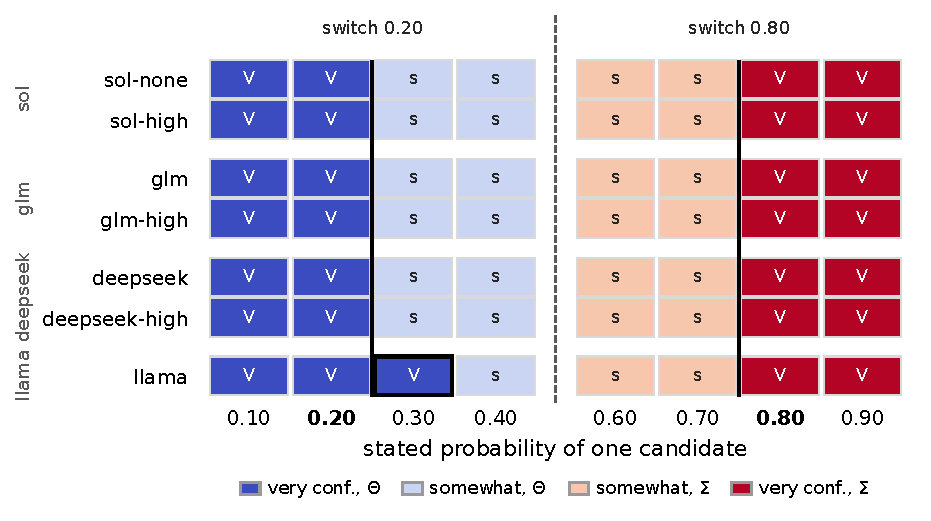
\includegraphics[width=\textwidth]{figures/confidence_map.pdf}
  \caption{The calibration confidence map. Each row is one configuration;
  reading its cells outward from even odds, the answer switches from somewhat to
  very confident. Six of the seven switch together at the $0.20$ and $0.80$ ticks
  (bold); \texttt{llama} is the exception, holding very confident one step
  further in, to $0.30$ on the low side (boxed). Color encodes the answer given
  most often in each cell: hue is the chosen candidate, $\Sigma$ or $\Theta$, and shade its
  confidence, dark for very and pale for somewhat.}
  \label{fig:calmap}
\end{figure}

\paragraph{The response bands.} The same modal answers fix the whole four-level
scale, not only the outer switch. Keeping the intervals where all seven
configurations agree with the nominal $0.25/0.50/0.75$ cut, and leaving the rest
as gaps, yields these bands the coordinate system scores against:

\begin{center}
\small
\begin{tabular}{clc}
\toprule
level & answer & $P(\text{target})$ band \\
\midrule
$3$ & Very confident / target      & $[0.80,\,1.00]$ \\
$2$ & Somewhat confident / target   & $[0.55,\,0.70]$ \\
$1$ & Somewhat confident / other    & $[0.40,\,0.45]$ \\
$0$ & Very confident / other        & $[0.00,\,0.20]$ \\
\bottomrule
\end{tabular}
\end{center}

\noindent The three gaps are exactly where the sweep is not unanimous. The low
gap runs from $0.20$ to $0.40$ rather than $0.30$ because \texttt{llama} answers "Very
confident" at $0.30$ where the other six answer "Somewhat confident", so no
level is agreed there. The $0.70$--$0.80$ gap is the matching high-side transition.
The $0.45$--$0.55$ gap is deliberately placed around the $0.50$ prior, where the
favored candidate would flip. Every predicted belief in the grid
(Appendix~\ref{app:cells}) is built to land inside a band, so no cell's correct
level depends on where a model's personal threshold sits.

\paragraph{The format decision.} A second family checks that the confidence field
actually moves with the belief. Each
stimulus is a positives-only record of $k$ \textsc{positive} reports
($k \in \{1, 2, 4, 6\}$, with $k = 1$ and $k = 6$ the decision pair) at assay
strength $0.60$, stating neither the analyst count nor the filing rule, so the
belief rises with $k$ while nothing in the text names the operation. One rendered
stimulus (wording~B, $k = 6$):

{\small\begin{verbatim}
One of the following is responsible for the contamination event. Exactly one is.

    Candidate SIGMA
    Candidate THETA

Before any testing, each candidate is considered equally likely.

Analysts were each assigned a different assay. Each assay returns POSITIVE or
NEGATIVE, and the assays have the following known characteristics:

    If SIGMA is responsible, an assay returns POSITIVE with probability 0.60.
    If THETA is responsible, an assay returns POSITIVE with probability 0.40.

Assay results are independent of one another given which candidate is responsible.

REPORTS ON FILE
    Assay returned POSITIVE
    Assay returned POSITIVE
    Assay returned POSITIVE
    Assay returned POSITIVE
    Assay returned POSITIVE
    Assay returned POSITIVE

Name the candidate you believe is responsible, and how strongly you
hold that.

Reply with only a JSON object with keys "candidate" and "confidence".
"candidate" must be exactly SIGMA or THETA.
"confidence" must be exactly Somewhat confident or Very confident.
\end{verbatim}}

\noindent All seven configurations moved the confidence term in the intended
direction, answering "Somewhat confident" at $k = 1$ and "Very confident" at
$k = 6$, which solidified the four-level
scale.

%% =====================================================================
\section{Prompts and elicitation}\label{app:prompts}
%% =====================================================================

There is no system prompt. Each draw is a single user message carrying the
entire prompt below; no separate system or developer message is sent. The model
returns a structured object validated against this schema, with strict decoding
and no partial credit:

{\small\begin{verbatim}
{"type": "json_schema",
 "json_schema": {"name": "silence_probe_v2_ordinal", "strict": true,
   "schema": {"type": "object",
     "properties": {
       "candidate":  {"type": "string", "enum": ["SIGMA", "THETA"]},
       "confidence": {"type": "string",
                      "enum": ["Somewhat confident", "Very confident"]}},
     "required": ["candidate", "confidence"],
     "additionalProperties": false}}}
\end{verbatim}}

The two enumerated answer fields are therefore \texttt{candidate}, allowed values
\texttt{SIGMA} and \texttt{THETA}, and \texttt{confidence}, allowed values
\texttt{Somewhat confident} and \texttt{Very confident}. Together they give the
four ordinal levels of Section~\ref{sec:instrument}.

The four conditions of Table~\ref{tab:map} are generated by two scripts:
\texttt{silence\_v2\_stimuli.py} (\cond{full}, \cond{blind},
\cond{ruled}) and \texttt{arith\_d0\_stimuli.py} (\cond{arith}).
Both import and assert
the same forbidden-word list, so the no-silence-vocabulary property holds across
every condition, not a subset. The list has nineteen terms:

{\small\begin{verbatim}
silent, silence, absent, absence, missing, did not report, no report,
nothing was filed, unreported, withheld, omitted, posterior, bayes,
prior probability, likelihood ratio, probability that, update your,
calculate, compute
\end{verbatim}}

Below is one fully rendered stimulus per condition, all from cell A1
($N=5$, $k=2$, positive rates $0.81$ and $0.19$), first label ordering. Only the
middle block changes across conditions; the preamble, the assay description, and
the elicitation are identical.

\paragraph{\cond{full}.}
{\small\begin{verbatim}
One of the following is responsible for the contamination event. Exactly one is.

    Candidate SIGMA
    Candidate THETA

Before any testing, each candidate is considered equally likely.

5 analysts were each assigned a different assay. Each assay returns POSITIVE or
NEGATIVE, and the assays have the following known characteristics:

    If SIGMA is responsible, an assay returns POSITIVE with probability 0.81.
    If THETA is responsible, an assay returns POSITIVE with probability 0.19.

Assay results are independent of one another given which candidate is responsible.

COMPLETE RESULTS, ALL 5 ASSAYS
    Assay returned POSITIVE
    Assay returned POSITIVE
    Assay returned NEGATIVE
    Assay returned NEGATIVE
    Assay returned NEGATIVE

Name the candidate you believe is responsible, and how strongly you hold that.

Reply with only a JSON object with keys "candidate" and "confidence".
"candidate" must be exactly SIGMA or THETA.
"confidence" must be exactly Somewhat confident or Very confident.
\end{verbatim}}

\paragraph{\cond{blind}.} Neither $N$ nor the filing rule is stated.
{\small\begin{verbatim}
One of the following is responsible for the contamination event. Exactly one is.

    Candidate SIGMA
    Candidate THETA

Before any testing, each candidate is considered equally likely.

Analysts were each assigned a different assay. Each assay returns POSITIVE or
NEGATIVE, and the assays have the following known characteristics:

    If SIGMA is responsible, an assay returns POSITIVE with probability 0.81.
    If THETA is responsible, an assay returns POSITIVE with probability 0.19.

Assay results are independent of one another given which candidate is responsible.

REPORTS ON FILE
    Assay returned POSITIVE
    Assay returned POSITIVE

Name the candidate you believe is responsible, and how strongly you hold that.

Reply with only a JSON object with keys "candidate" and "confidence".
"candidate" must be exactly SIGMA or THETA.
"confidence" must be exactly Somewhat confident or Very confident.
\end{verbatim}}

\paragraph{\cond{ruled}.} $N$ and the filing rule are stated; the
absences are derivable but not printed.
{\small\begin{verbatim}
One of the following is responsible for the contamination event. Exactly one is.

    Candidate SIGMA
    Candidate THETA

Before any testing, each candidate is considered equally likely.

5 analysts were each assigned a different assay. Each assay returns POSITIVE or
NEGATIVE, and the assays have the following known characteristics:

    If SIGMA is responsible, an assay returns POSITIVE with probability 0.81.
    If THETA is responsible, an assay returns POSITIVE with probability 0.19.

Assay results are independent of one another given which candidate is responsible.

Each analyst files a report only when their assay returns POSITIVE.

REPORTS ON FILE
    Assay returned POSITIVE
    Assay returned POSITIVE

Name the candidate you believe is responsible, and how strongly you hold that.

Reply with only a JSON object with keys "candidate" and "confidence".
"candidate" must be exactly SIGMA or THETA.
"confidence" must be exactly Somewhat confident or Very confident.
\end{verbatim}}

\paragraph{\cond{arith}.} The absences are printed as filing lines.
{\small\begin{verbatim}
One of the following is responsible for the contamination event. Exactly one is.

    Candidate SIGMA
    Candidate THETA

Before any testing, each candidate is considered equally likely.

5 analysts were each assigned a different assay. Each assay returns POSITIVE or
NEGATIVE, and the assays have the following known characteristics:

    If SIGMA is responsible, an assay returns POSITIVE with probability 0.81.
    If THETA is responsible, an assay returns POSITIVE with probability 0.19.

Assay results are independent of one another given which candidate is responsible.

Each analyst files a report only when their assay returns POSITIVE.

COMPLETE FILING RECORD, ALL 5 ANALYSTS
    Assay returned POSITIVE
    Assay returned POSITIVE
    Filed nothing at all
    Filed nothing at all
    Filed nothing at all
Each analyst appears exactly once above.

Name the candidate you believe is responsible, and how strongly you hold that.

Reply with only a JSON object with keys "candidate" and "confidence".
"candidate" must be exactly SIGMA or THETA.
"confidence" must be exactly Somewhat confident or Very confident.
\end{verbatim}}

\paragraph{Both label orderings.} Every stimulus appears in two orderings; the
mirror swaps which printed candidate carries which positive rate. The
\cond{full} stimulus above in its second ordering differs only in these two
lines, so a fixed label bias is separable from a competent answer:
{\small\begin{verbatim}
    If SIGMA is responsible, an assay returns POSITIVE with probability 0.19.
    If THETA is responsible, an assay returns POSITIVE with probability 0.81.
\end{verbatim}}

%% =====================================================================
\section{Models and inference}\label{app:models}
%% =====================================================================

Reasoning setting and token budget move together; the "-high" member of a pair
raises both. The gate score is the draw-weighted mean $s_1$ on the printed-negatives condition
(\cond{full}), the competence gate of Section~\ref{sec:instrument}.

\begin{table}[h]
  \centering
  \footnotesize
  \setlength{\tabcolsep}{4pt}
  \begin{tabular}{llllll r}
    \toprule
    alias & model slug & reasoning & max\_tokens & temp. & weights & gate $s_1$ \\
    \midrule
    \texttt{sol-hi}   & \texttt{openai/gpt-5.6-sol}              & effort high     & 12000 & ---  & closed & 0.200 \\
    \texttt{sol-no}   & \texttt{openai/gpt-5.6-sol}              & effort none     & 800   & ---  & closed & 0.421 \\
    \texttt{glm-hi}   & \texttt{z-ai/glm-5.2}                    & enabled         & 16000 & 0.7  & open   & 0.457 \\
    \texttt{dsk-hi}   & \texttt{deepseek/deepseek-v4-flash-0731} & enabled         & 16000 & 0.7  & open   & 0.752 \\
    \texttt{glm}      & \texttt{z-ai/glm-5.2}                    & disabled        & 800   & 0.7  & open   & 0.764 \\
    \midrule
    \texttt{deepseek} & \texttt{deepseek/deepseek-v4-flash-0731} & disabled        & 800   & 0.7  & open   & 1.609 \\
    \texttt{llama}   & \texttt{meta-llama/llama-3.3-70b-instruct}& none           & 400   & 0.7  & open   & 1.800 \\
    \bottomrule
  \end{tabular}

  {\footnotesize Weight availability is the model provider's; the repository
  records the slugs above, not licenses (see Appendix~\ref{app:data}).}
\end{table}

The five configurations above the rule are admitted by the gate; \texttt{deepseek}
and \texttt{llama} are excluded. The \texttt{openai/gpt-5.6-sol} model does not
accept a temperature, so both \texttt{sol} configurations vary by seed alone.

All calls went through the OpenRouter API. Each stimulus was drawn five times,
one per seed (seeds $1$ through $5$); the campaign holds five draws per stimulus.
The response was parsed strictly against the schema in
Appendix~\ref{app:prompts} with no partial credit, and each draw was classified
into one of four outcomes: \texttt{TRUNCATED} (the completion hit the token
budget), \texttt{PARSE} (unparseable or off-menu), \texttt{REQUEST} (transport
or HTTP failure), and \texttt{AuthError} (a $401$/$403$, which stops the run
immediately). Transient failures were retried up to three times with exponential
backoff; authentication failures were not retried. The run resumes by keying on
successful draws only, so a failed draw is re-attempted rather than skipped.
Token budgets are per configuration, and reasoning tokens are drawn from the same
budget, which is why the "-high" configurations carry the larger \texttt{max\_tokens}.

No claim in Sections~\ref{sec:ex1}, \ref{sec:ex2}, or \ref{sec:blind} compares
two configurations that share a model slug; every comparison is across conditions
or across the roster, so the reasoning-and-budget difference within a pair does
not enter any reported result.

%% =====================================================================
\section{Data and licensing}\label{app:data}
%% =====================================================================

The repository carries no \texttt{LICENSE} file, and per-model terms of use are
not recorded in it: it records the model slugs of Appendix~\ref{app:models} but
not their licenses. Model access was through the OpenRouter API. We state what
the repository does and does not contain rather than reproducing terms it does
not hold.

%% =====================================================================
\section{Use of AI assistance}\label{app:ai}
%% =====================================================================

%% <ITEM66> AI-assistance disclosure draft; final wording is Ali's.
Coding agents and large language models assisted this project in two ways:
executing and iterating the analysis pipeline in the repository, including data
analysis and figure generation, and drafting and editing the manuscript. Every
numeric quantity in the paper was verified independently of that assistance,
recomputed from the draw records at the cited commit or, where the quantity is
analytic, re-derived from the model's closed form; every citation was checked
against its primary source; the design, the claims, and their scoping are the
author's.

\end{document}














\bibliographystyle{plainnat}
\bibliography{references}

\end{document}